%%%%%%%%%%%%%%%%%%%%%%%%%%%%%%%%%%%%%%%%%%%%%%%%%%%%%%
% A Beamer template for HKUST (GZ)                   %
% Based on THU beamer theme                          %
% Author: Yuxuan HU                                  %
% Date: Aug 2024                                    %
% LPPL Licensed.                                     %
%%%%%%%%%%%%%%%%%%%%%%%%%%%%%%%%%%%%%%%%%%%%%%%%%%%%%%

\documentclass[serif, aspectratio=169]{beamer}
%\documentclass[serif]{beamer}  % for 4:3 ratio
\usepackage[T1]{fontenc} 
\usepackage{fourier} % see "http://faq.ktug.org/wiki/uploads/MathFonts.pdf" for other options
\usepackage{hyperref}
\usepackage{latexsym,amsmath,xcolor,multicol,booktabs,calligra}
\usepackage{graphicx,pstricks,listings,stackengine}
\usepackage{lipsum}
\usepackage{parskip}

\author{MAS}
\title{KANs and DeepOKANs}
\subtitle{Brief Introduction}
\institute{
    \\
    IISc, Bengaluru\\
}
\date{\small \today}
\usepackage{HKUSTstyle}

% defs
\def\cmd#1{\texttt{\color{red}\footnotesize $\backslash$#1}}
\def\env#1{\texttt{\color{blue}\footnotesize #1}}
% set colors
\definecolor{hkustyellow}{RGB}{167, 131, 55}
\definecolor{hkustblue}{RGB}{0, 56, 116}
\definecolor{hkustred}{RGB}{209, 51, 59}


\lstset{
    basicstyle=\ttfamily\small,
    keywordstyle=\bfseries\color{deepblue},
    emphstyle=\ttfamily\color{deepred},    % Custom highlighting style
    stringstyle=\color{deepgreen},
    numbers=left,
    numberstyle=\small\color{halfgray},
    rulesepcolor=\color{red!20!green!20!blue!20},
    frame=shadowbox,
}

%- --- --- --- --- --- --- --- --- --- --- --- --- --- --- --- 
\begin{document}

\begin{frame}
    \titlepage
    \vspace*{-0.6cm}
    \begin{figure}[htpb]
        \begin{center}
            
\includegraphics[keepaspectratio, scale=0.02]{unilogo.png}
        \end{center}
    \end{figure}
\end{frame}

\begin{frame}
    \tableofcontents[sectionstyle=show,
        subsectionstyle=show/shaded/hide,
        subsubsectionstyle=show/shaded/hide]
\end{frame}

% Introduction --- --- --- --- --- --- --- --- --- --- --- --- 

\section{Introduction to Data Fitting}
\begin{frame}{Background and Motivation}
    \frametitle<presentation>{Representing Smooth Functions}
    %attaching a picture from umar jamil
    \begin{figure}
        \centering
        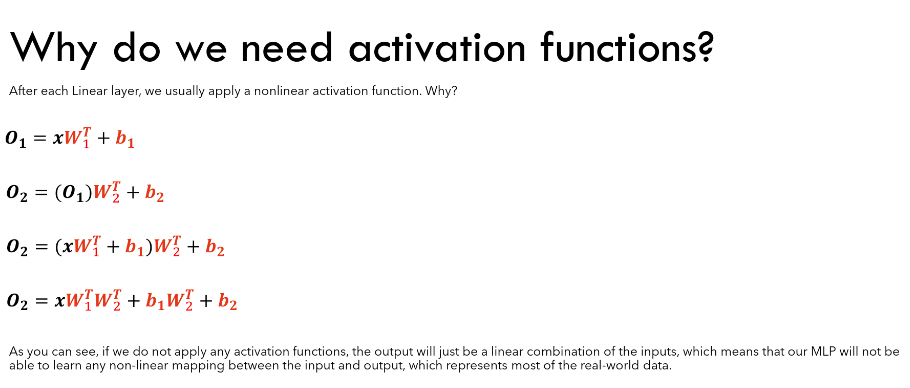
\includegraphics[height=6cm]{datafit.png}
    \end{figure}
    % \begin{block}{}
    %     \begin{itemize}
    %         \item show the main arguments and resuts of your work
    %         \item produce interest to read the full paper/report
    %         \item goal: be educational and also entertaining
    %     \end{itemize}
    % \end{block}
    % \begin{block}{Advantages of using \LaTeX ~with the beamer package:}
    %     \begin{itemize}
    %         \item very easy if the report is already written in \LaTeX
    %         \item different themes which are usable in practice
    %         \item possibility to create handouts using \emph{beamerarticle}
    %     \end{itemize}
    % \end{block}
\end{frame}

\begin{frame}{Background and Motivation}
    \frametitle<presentation>{Representing Smooth Functions}
    %attaching a picture from umar jamil
    \begin{figure}
        \centering
        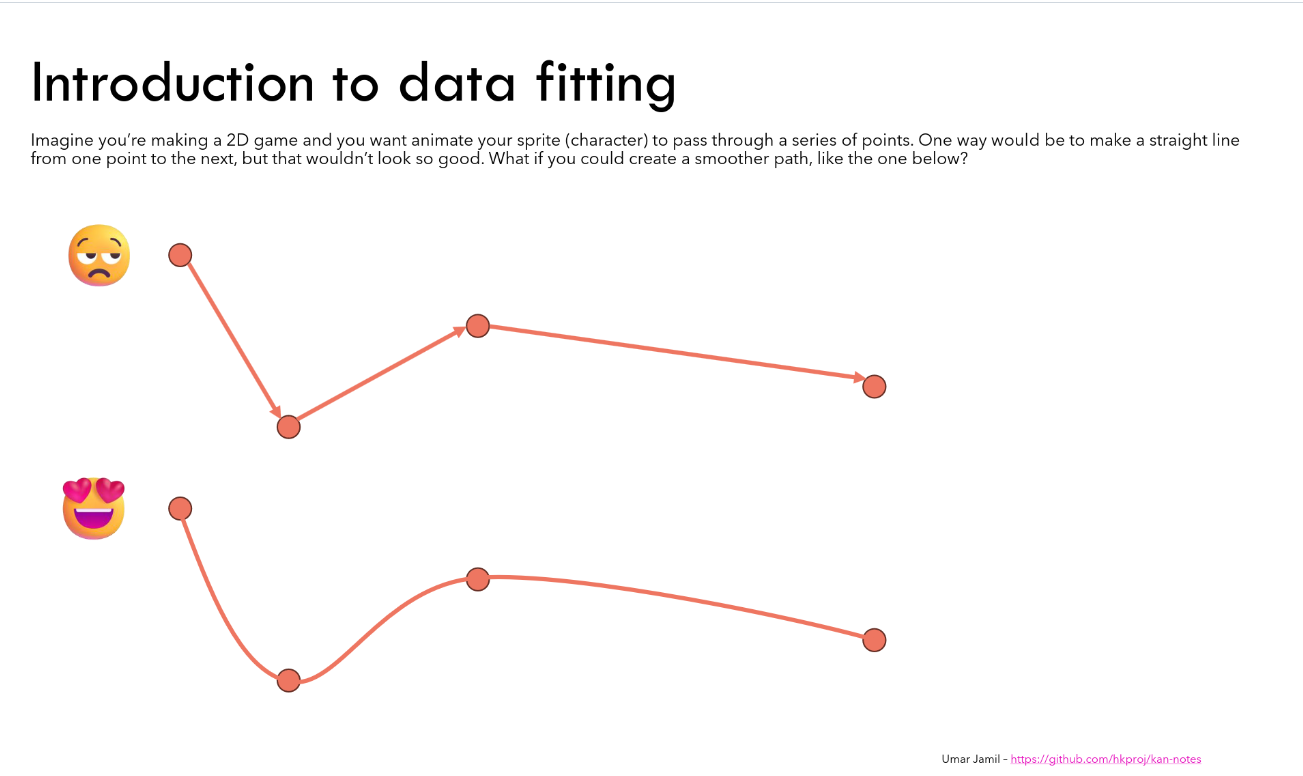
\includegraphics[height=7cm]{smooth.png}
    \end{figure}
\end{frame}
\begin{frame}{Background and Motivation}
    \frametitle<presentation>{Representing Smooth Functions}
    %attaching a picture from umar jamil
    \begin{figure}
        \centering
        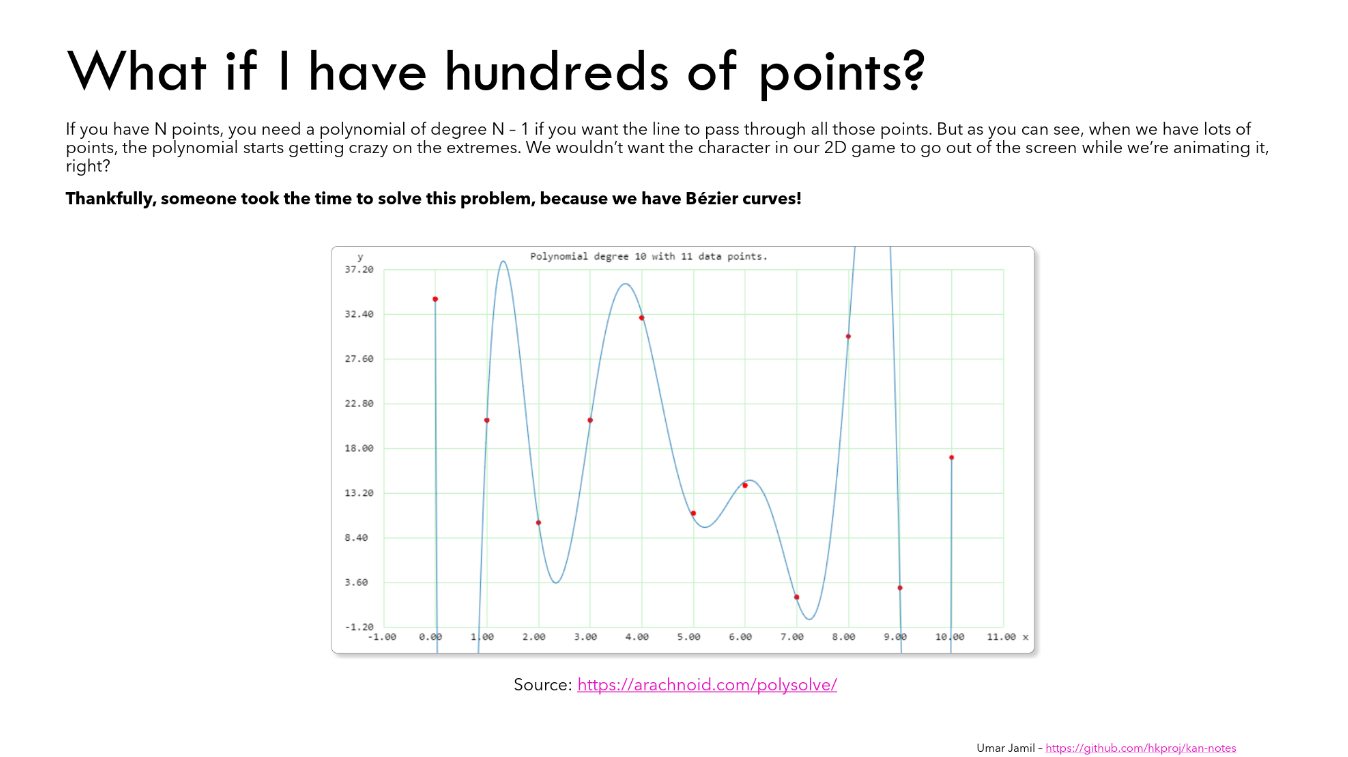
\includegraphics[height=7cm]{hund.png}
    \end{figure}
\end{frame}
\begin{frame}{Background and Motivation}
    \frametitle<presentation>{Representing Smooth Functions}
    %attaching a picture from umar jamil
    \begin{figure}
        \centering
        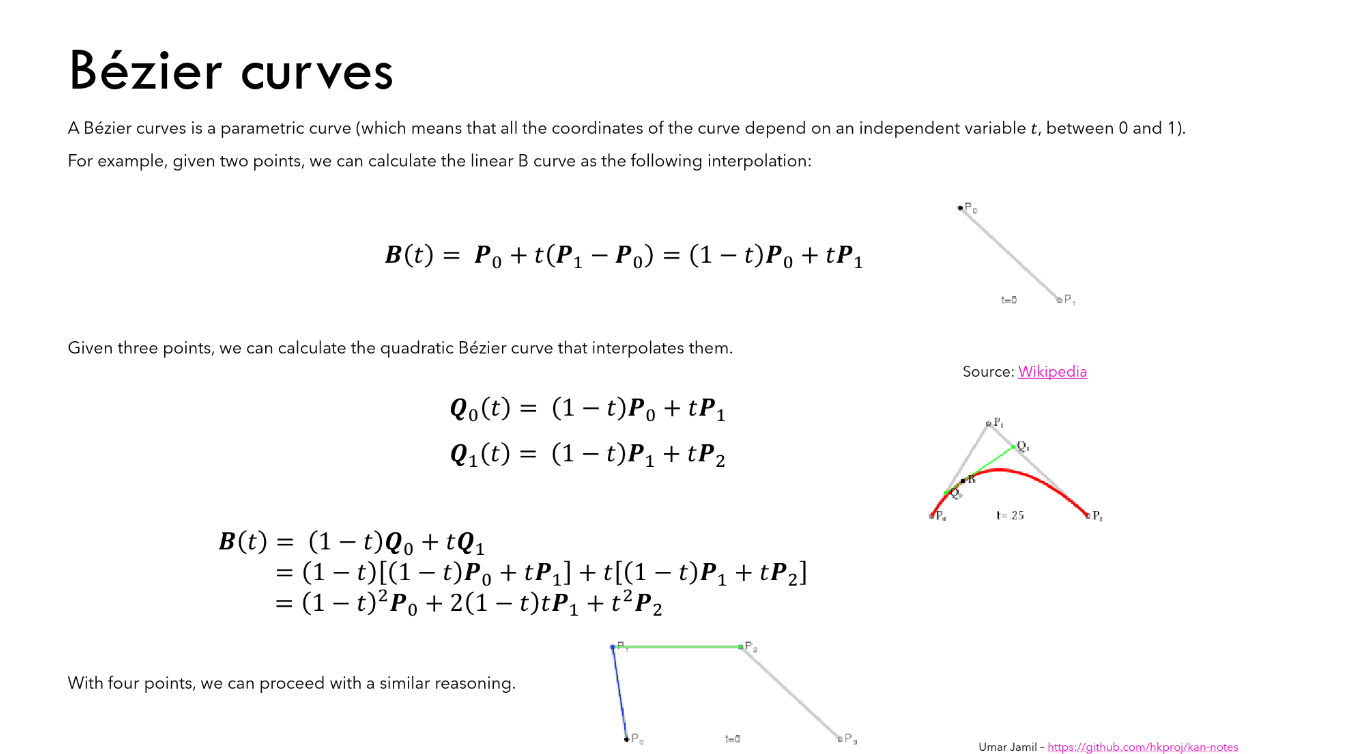
\includegraphics[height=7cm]{bezier.png}
    \end{figure}
\end{frame}
\begin{frame}{Background and Motivation}
    \frametitle<presentation>{Representing Smooth Functions}
    %attaching a picture from umar jamil
    \begin{figure}
        \centering
        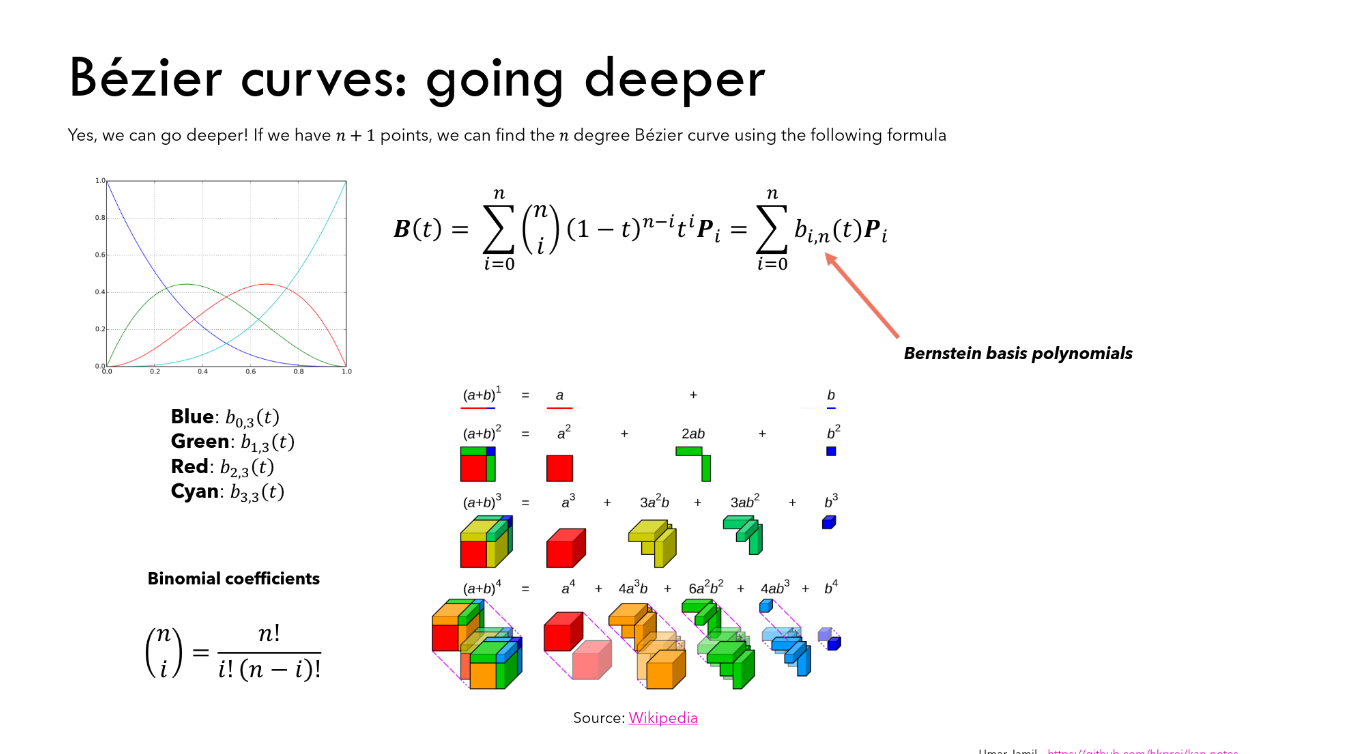
\includegraphics[height=7cm]{image.png}
    \end{figure}
\end{frame}
\begin{frame}{Background and Motivation}
    \frametitle<presentation>{Representing Smooth Functions}
    %attaching a picture from umar jamil
    \begin{figure}
        \centering
        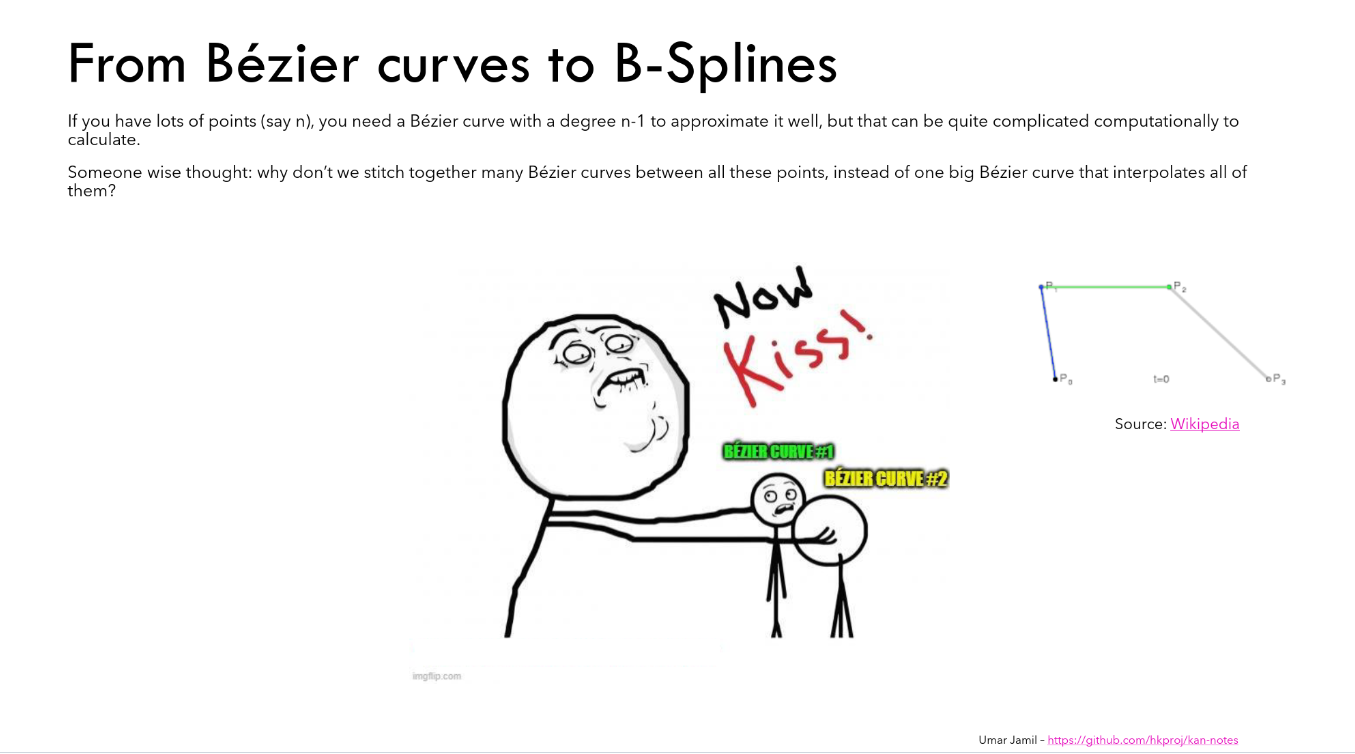
\includegraphics[height=7cm]{image copy.png}
    \end{figure}
\end{frame}
\begin{frame}{Background and Motivation}
    \frametitle<presentation>{Representing Smooth Functions}
    %attaching a picture from umar jamil
    \begin{figure}
        \centering
        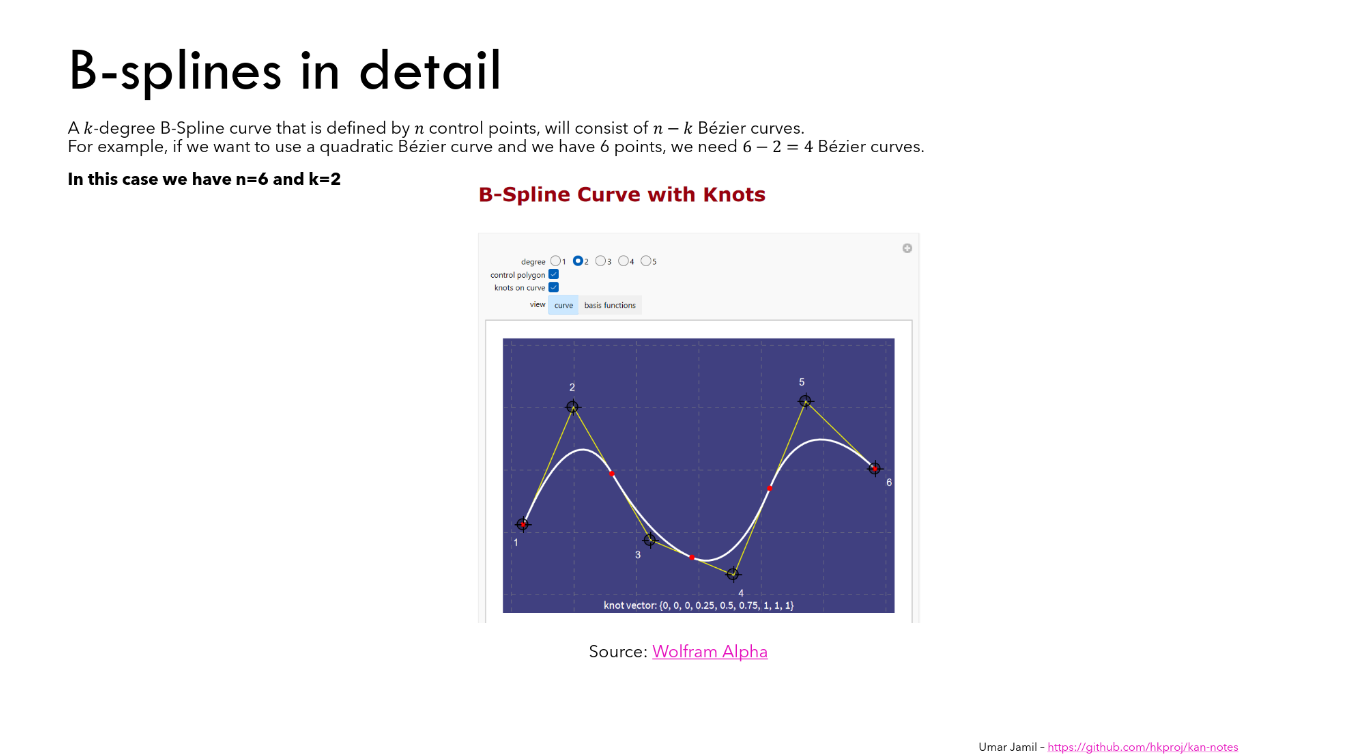
\includegraphics[height=7cm]{image copy 2.png}
    \end{figure}
\end{frame}
\begin{frame}{Background and Motivation}
    \frametitle<presentation>{Representing Smooth Functions}
    %attaching a picture from umar jamil
    \begin{figure}
        \centering
        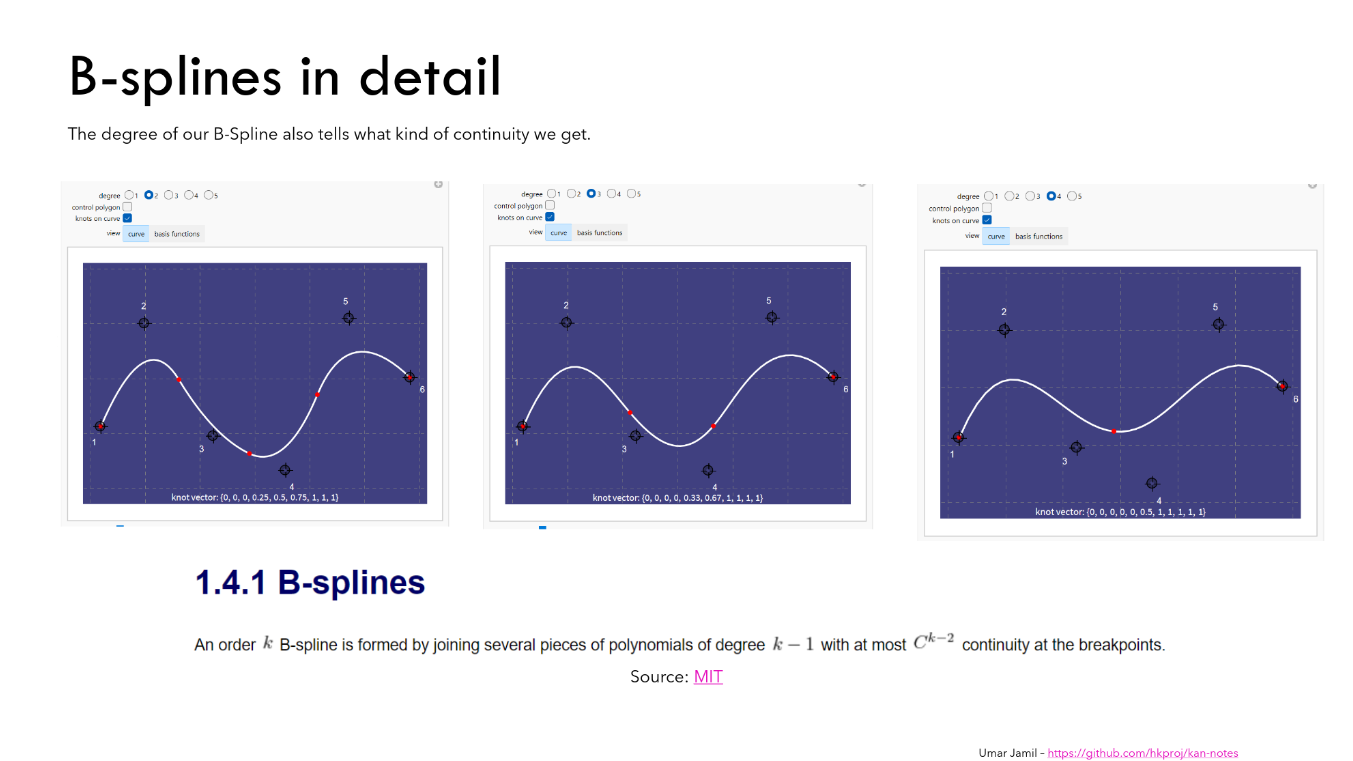
\includegraphics[height=7cm]{image copy 3.png}
    \end{figure}
\end{frame}
\begin{frame}{Background and Motivation}
    \frametitle<presentation>{Representing Smooth Functions}
    %attaching a picture from umar jamil
    \begin{figure}
        \centering
        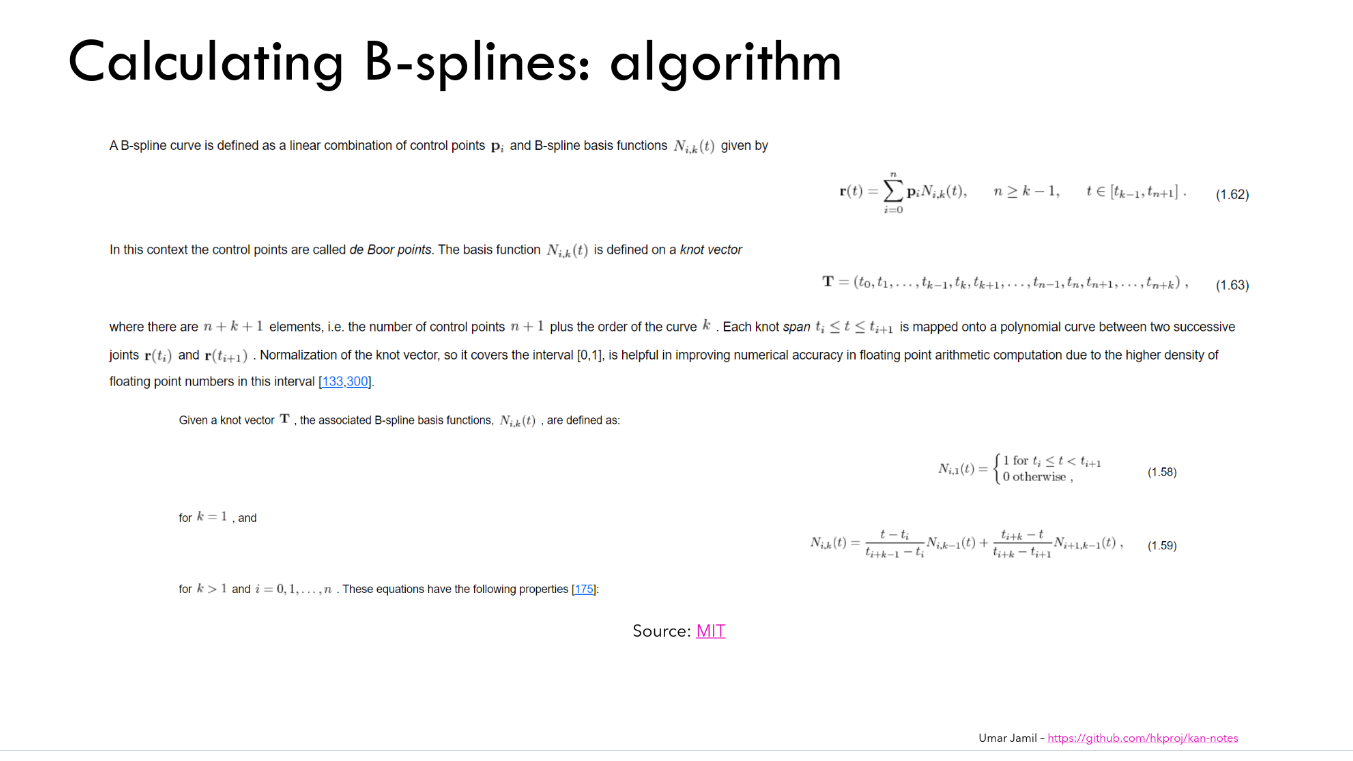
\includegraphics[height=7cm]{image copy 4.png}
    \end{figure}
\end{frame}
\begin{frame}{Background and Motivation}
    \frametitle<presentation>{Representing Smooth Functions}
    %attaching a picture from umar jamil
    \begin{figure}
        \centering
        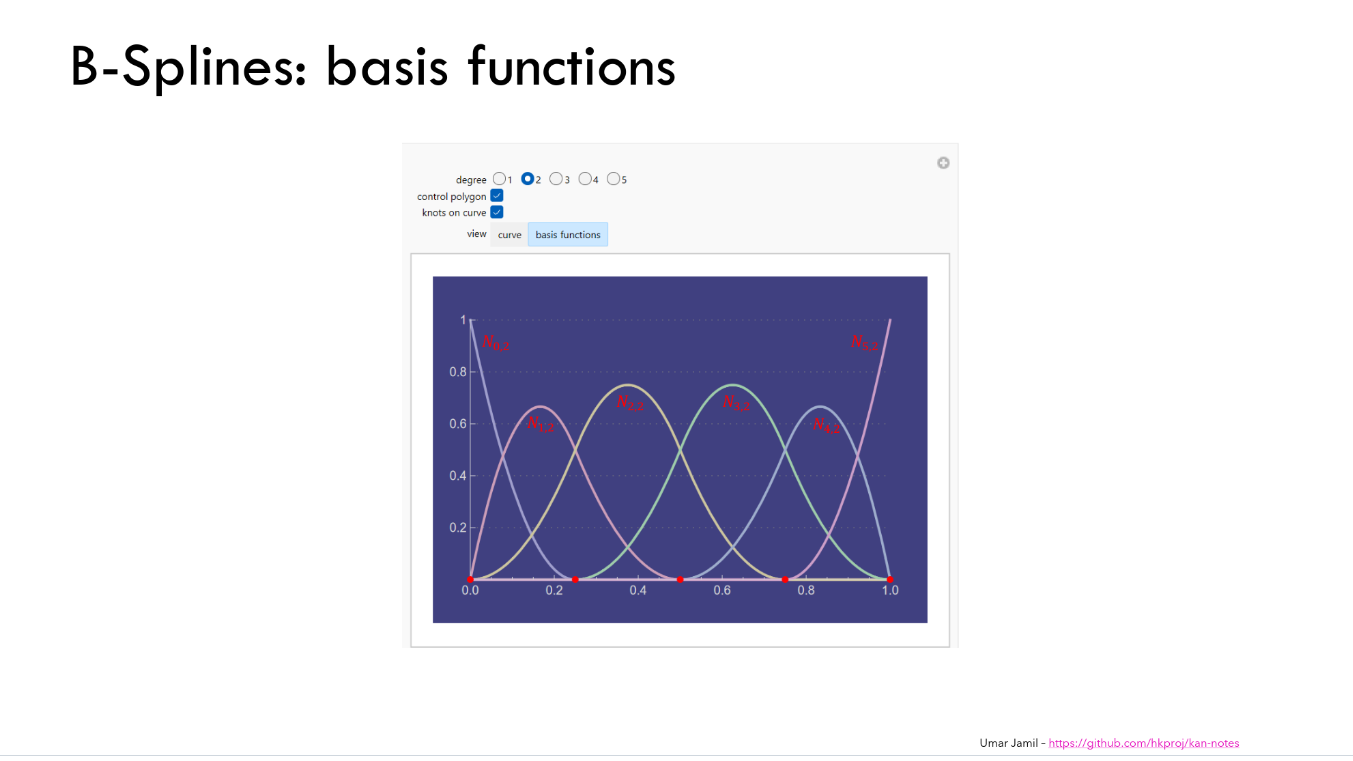
\includegraphics[height=7cm]{image copy 5.png}
    \end{figure}
\end{frame}
\begin{frame}{Background and Motivation}
    \frametitle<presentation>{Representing Smooth Functions}
    %attaching a picture from umar jamil
    \begin{figure}
        \centering
        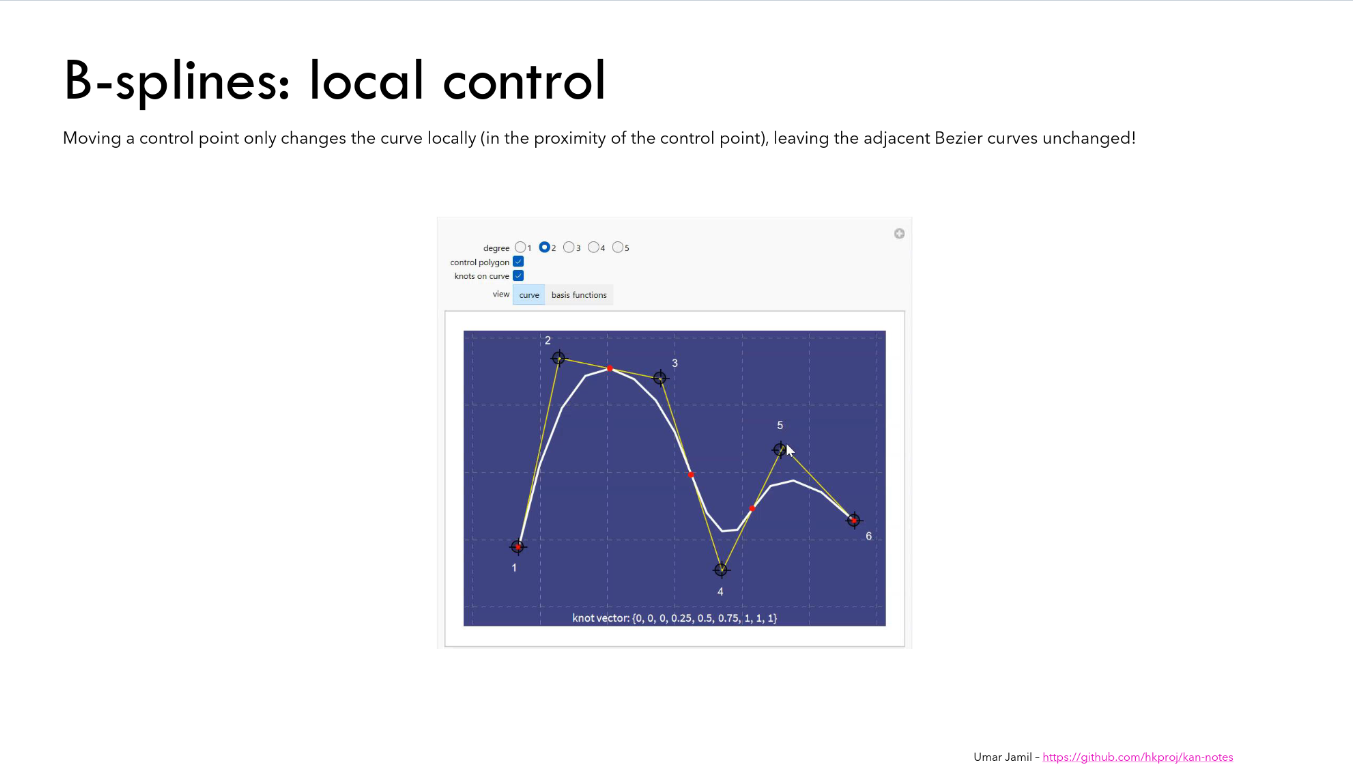
\includegraphics[height=7cm]{image copy 6.png}
    \end{figure}
\end{frame}
% Literature Review --- --- --- --- --- --- --- --- --- --- --- 
\section{Introduction to KAN}
\begin{frame}{Intro to KAN}
    \frametitle<presentation>{MLP vs KAN}
    %attaching a picture from umar jamil
    \begin{figure}
        \centering
        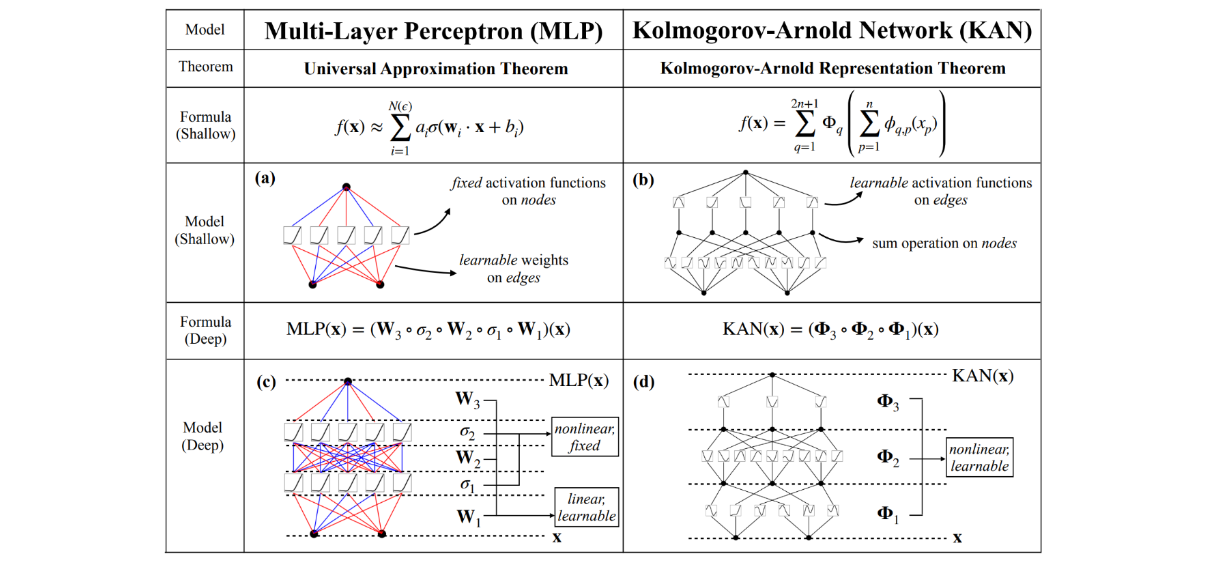
\includegraphics[height=6cm]{image copy 7.png}
    \end{figure}
\end{frame}
\begin{frame}{Intro to KAN}
    \frametitle<presentation>{Why KAN and not MLPs?}
    - \textbf{MLPs \& Nonlinear Approximation}: MLPs are widely used for nonlinear function approximation due to their expressive power (Universal Approximation Theorem), but they have drawbacks: low interpretability, less accuracy in low dimensions, and the curse of dimensionality (COD) in high dimensions.

    - \textbf{Introduction of KANs}: The paper introduces Kolmogorov-Arnold Networks (KANs), inspired by the Kolmogorov-Arnold representation theorem, as an alternative to MLPs.

    - \textbf{Previous Work}: Earlier research focused on depth-2, width-(2n + 1) networks, showing potential in breaking the COD empirically and theoretically, particularly with compositional function structures.

    - \textbf{New Approach}: This paper proposes deeper and wider network architectures, leveraging backpropagation for training, to enhance performance beyond the traditional depth-2, width-(2n + 1) representation.
\end{frame}
\begin{frame}{Intro to KAN}
    \frametitle<presentation>{KANs are a combo of MLPs and splines}
    - \textbf{Splines}: Accurate for low dimensions, easy to adjust locally and able to switch between different resolutions.(resolutions are the number of knots in the spline)
    But suffer from COD in high dimensions, unable to learn compositional structures

    - \textbf{MLPs}: suffer less from COD thanks to their feature learning, but are less accurate than splines in low dimensions,
    because of their inability to optimize univariate functions.

    To learn a function accurately,
    a model should not only learn the compositional structure (external degrees of freedom), but should
    also approximate well the univariate functions (internal degrees of freedom).

    Solution: KANs = MLPs(learns external dofs) + splines(learns internal dofs)
\end{frame}
\begin{frame}{Intro to KAN}
    \frametitle<presentation>{Brief Idea of Advantages of KANs}
    \begin{itemize}
        \item KANs can lead to
              accuracy and interpretability improvement over MLPs
        \item KANs can be made more accurate with grid extension
        \item KANs can beat the curse of dimensionality when there is a compositional structure in data, achieving better scaling laws than MLPs.
        \item PDE solutions can be approximated with KANs (Something we might want to research on)
        \item Two examples from mathematics (knot theory) and physics (Anderson localization) to
              demonstrate that KANs can be helpful “collaborators” for scientists to (re)discover math and phys-
              ical laws. \textbf{No Background hence skipped}
    \end{itemize}

\end{frame}
% Methods --- --- --- --- --- --- --- --- --- --- --- 
\section{KAT}
\begin{frame}{Kolmogorov-Arnold Represenation Theorem}
    \begin{figure}
        \centering
        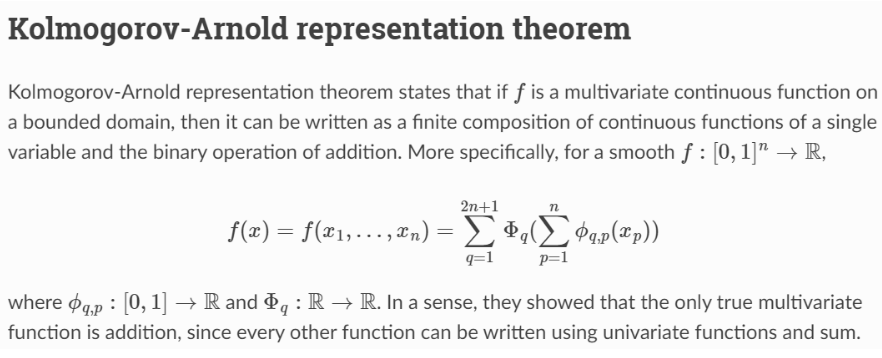
\includegraphics[height=6cm]{no3.png}
    \end{figure}
\end{frame}
\begin{frame}{KAT}
    \begin{figure}
        \centering
        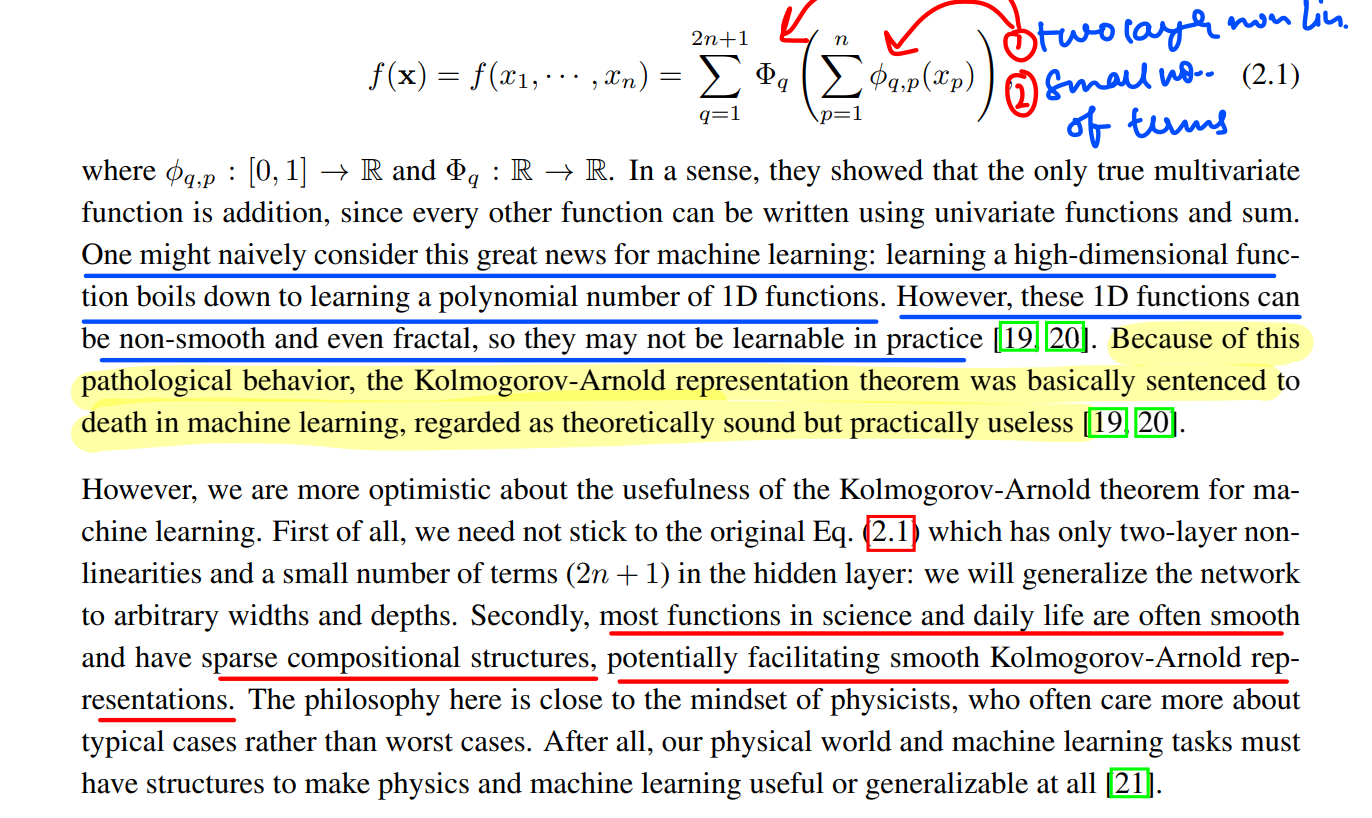
\includegraphics[height=7cm]{image copy 10.png}
    \end{figure}
\end{frame}
\begin{frame}{Mathematical Formulation}
    \begin{figure}
        \centering
        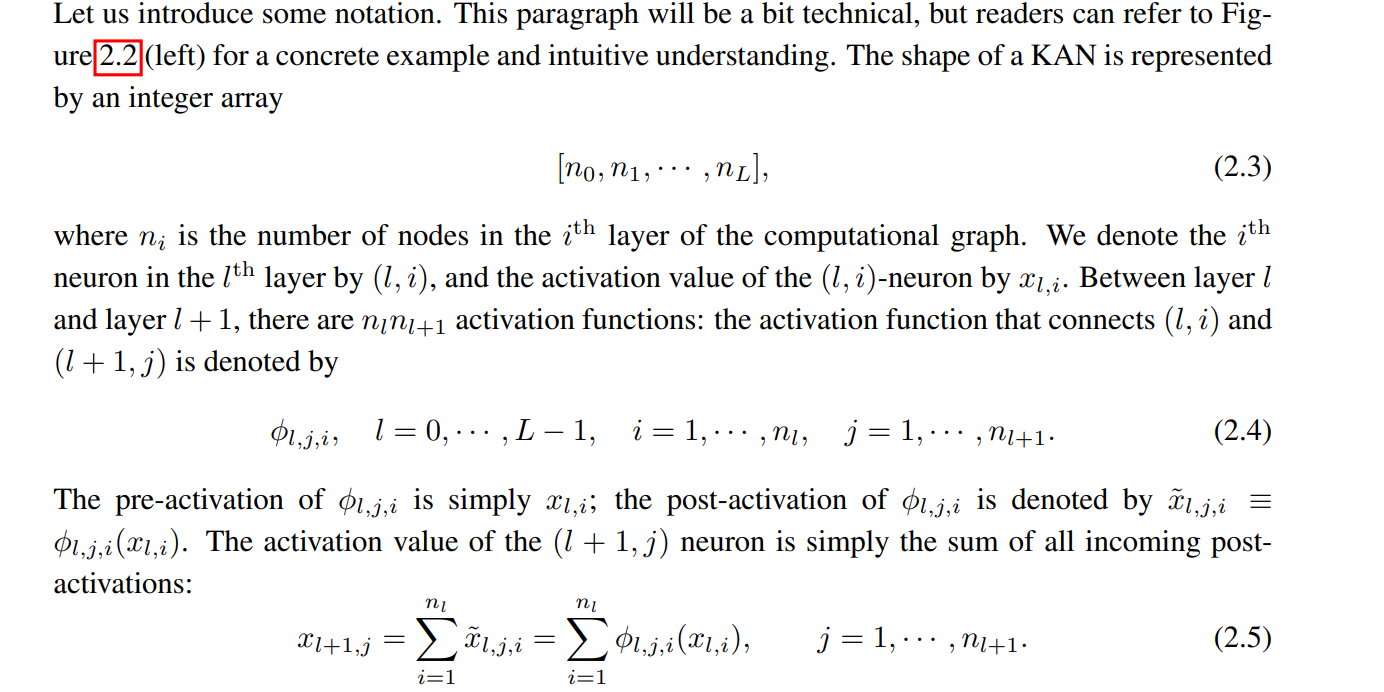
\includegraphics[height=6cm]{image copy 11.png}
    \end{figure}
\end{frame}
\begin{frame}{Mathematical Formulation}
    \begin{figure}
        \centering
        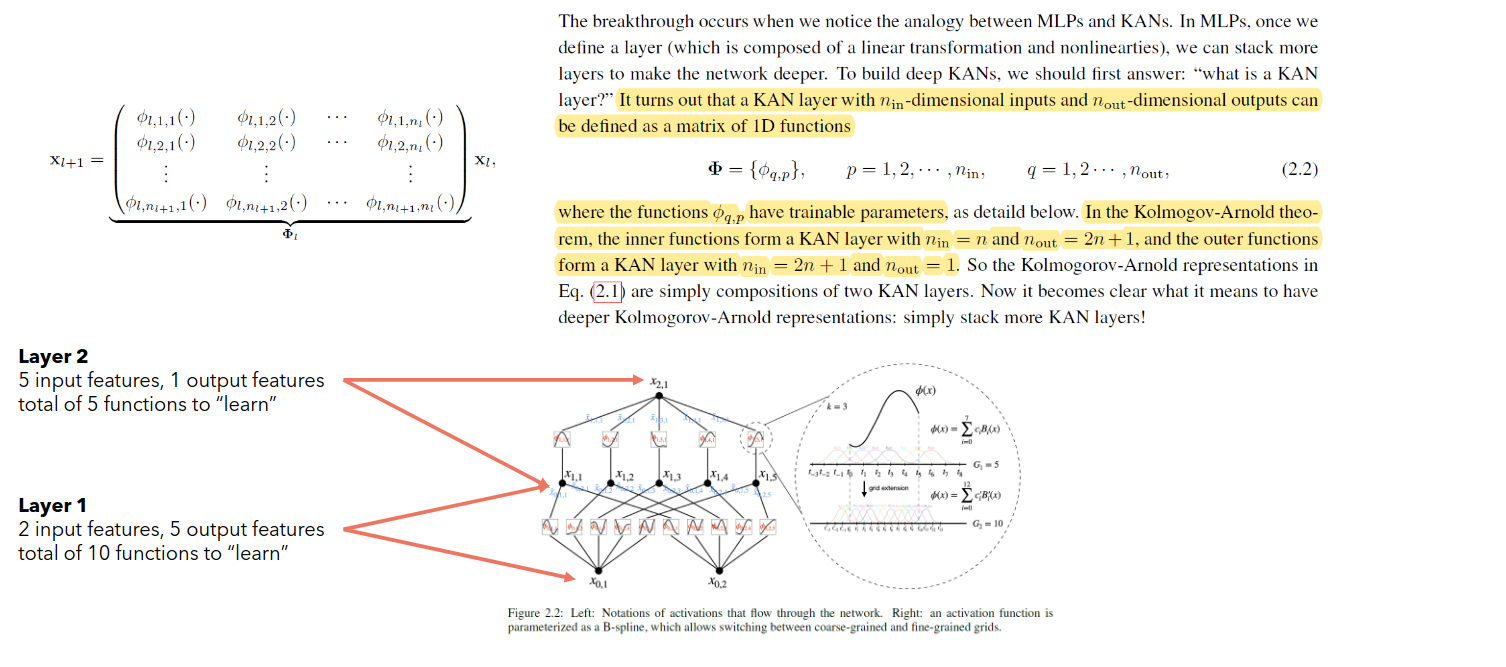
\includegraphics[height=7cm]{image copy 9.png}
    \end{figure}
\end{frame}
\begin{frame}{Example KAN}
    \begin{figure}
        \centering
        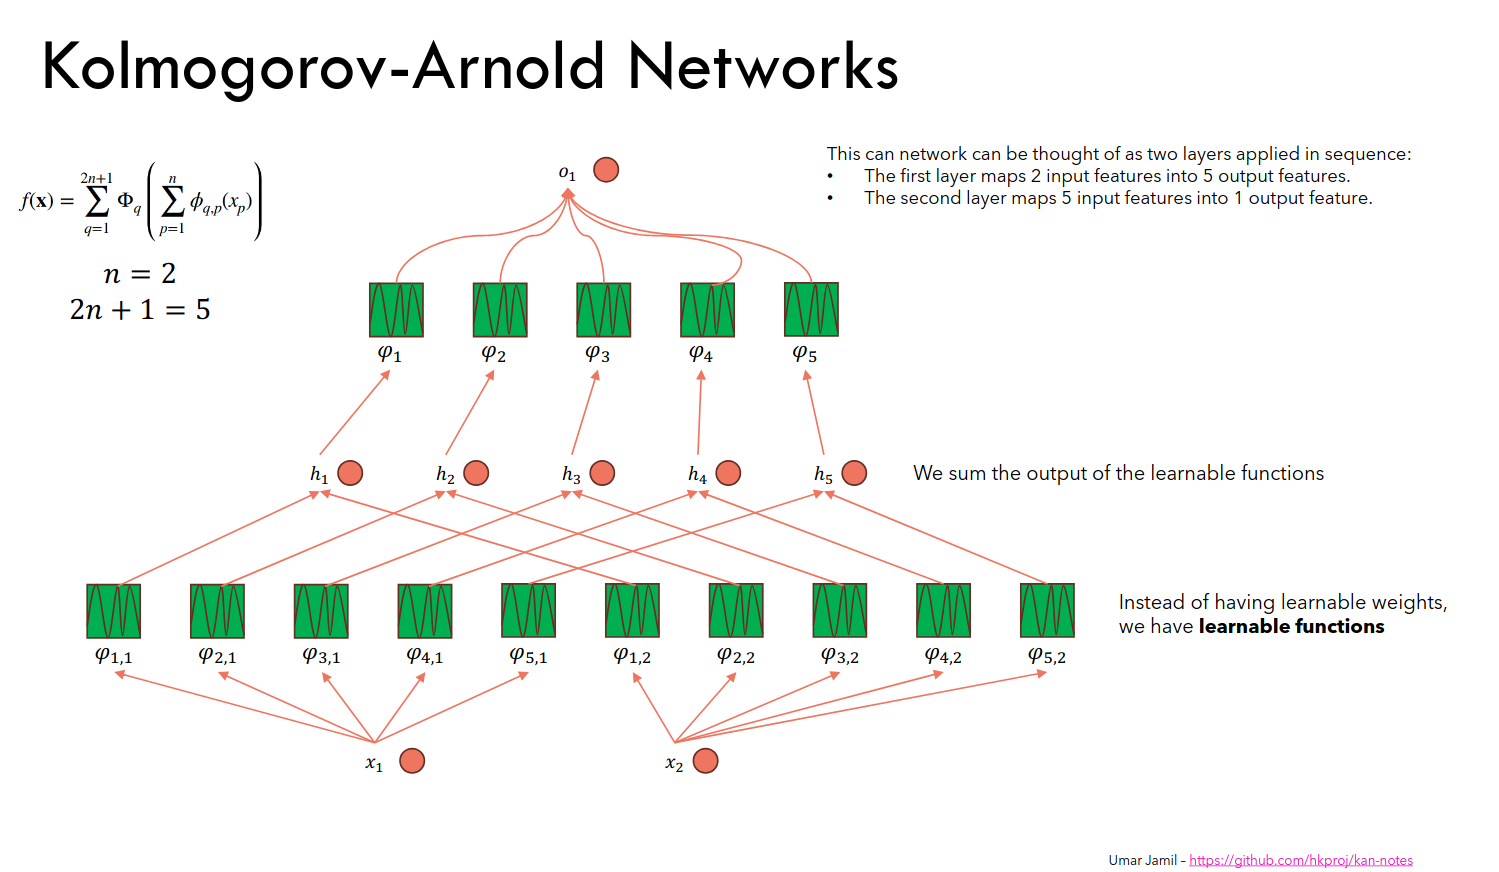
\includegraphics[height=7cm]{image copy 8.png}
    \end{figure}
\end{frame}
\begin{frame}{Example KAN}
    \begin{figure}
        \centering
        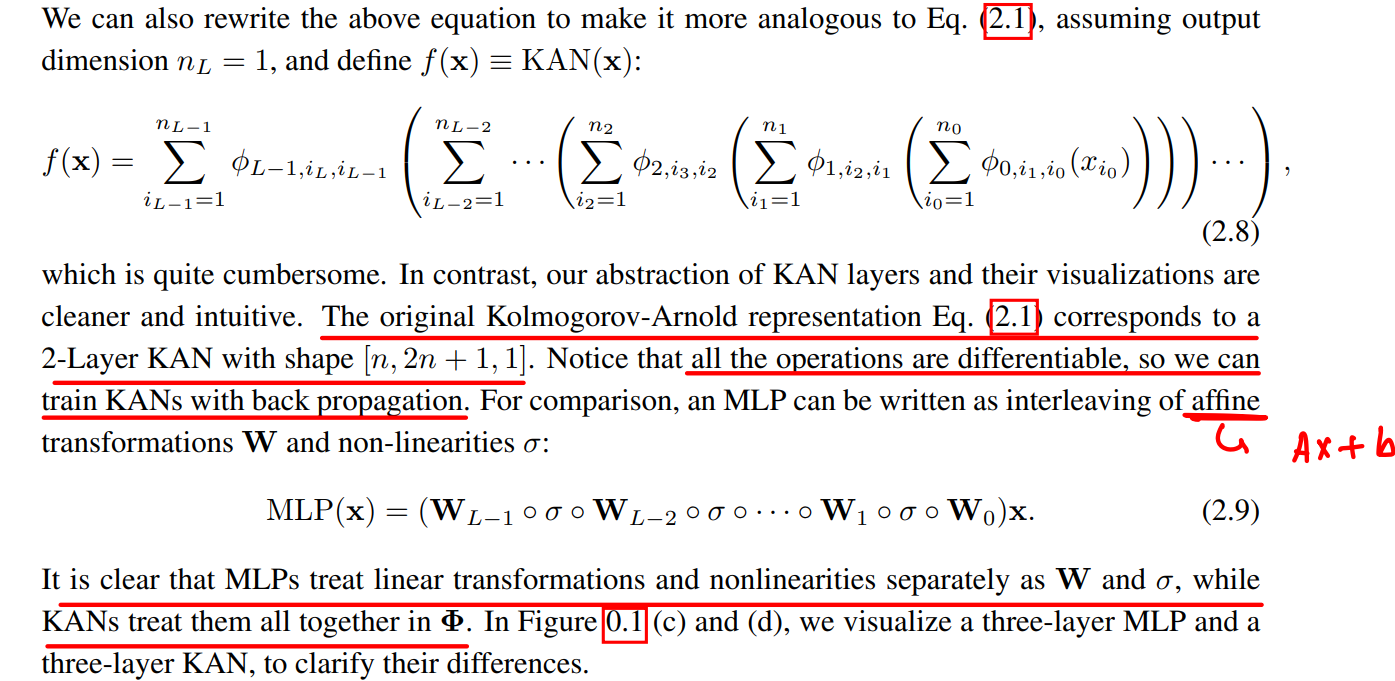
\includegraphics[height=7cm]{image copy 12.png}
    \end{figure}
\end{frame}
\begin{frame}
    \frametitle<presentation>{Implementation}
    \begin{figure}
        \centering
        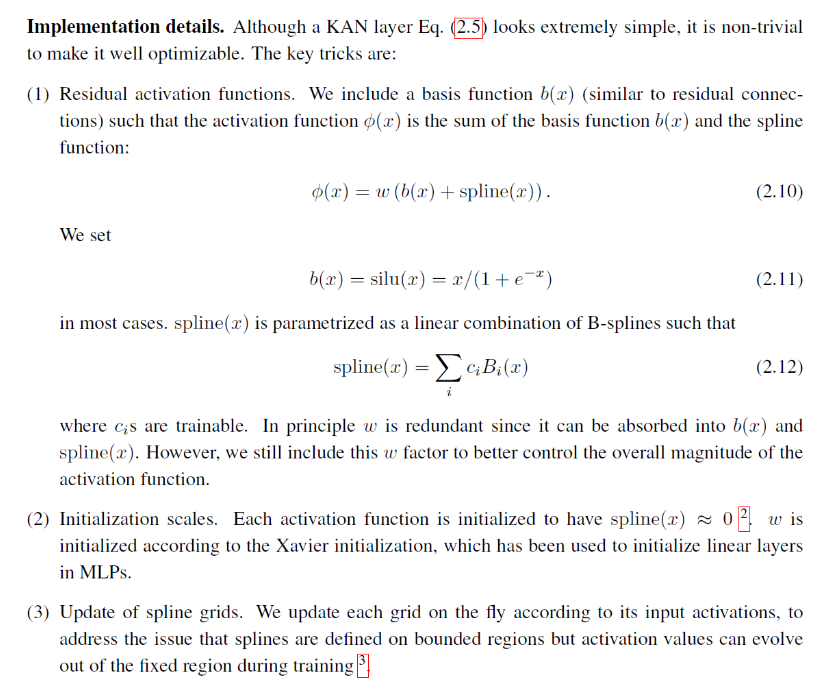
\includegraphics[height=7cm]{image copy 13.png}
    \end{figure}
\end{frame}
\begin{frame}
    \frametitle<presentation>{Parameter Count}
    \begin{figure}
        \centering
        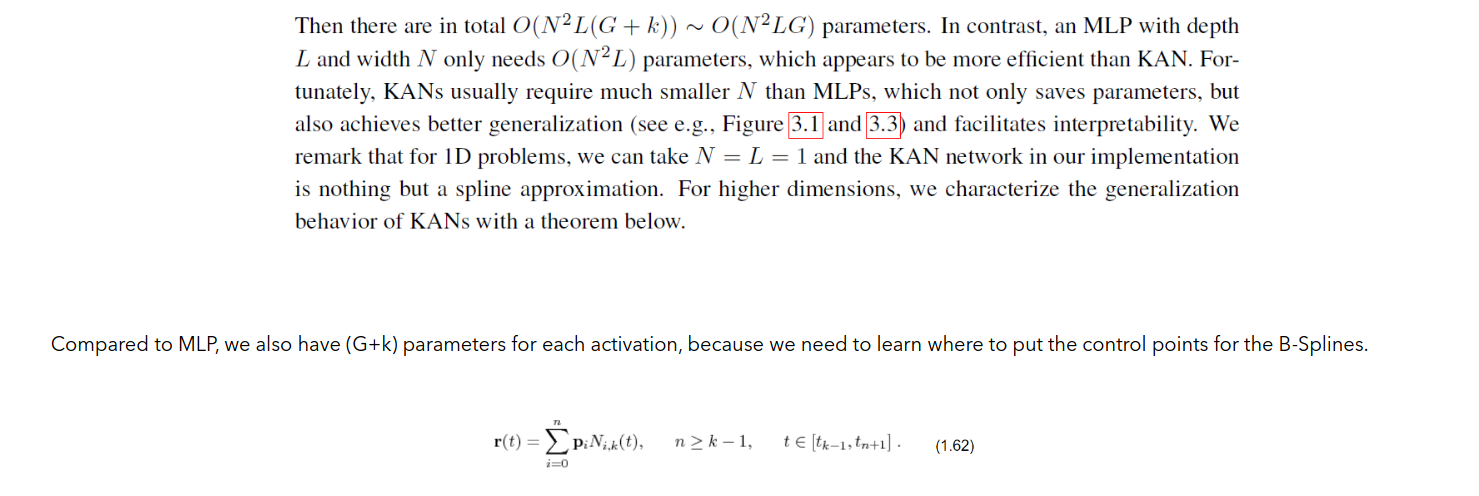
\includegraphics[height=5cm]{image copy 14.png}
    \end{figure}
\end{frame}
\begin{frame}
    \frametitle<presentation>{Approximation Theory, KAT}
    \begin{figure}
        \centering
        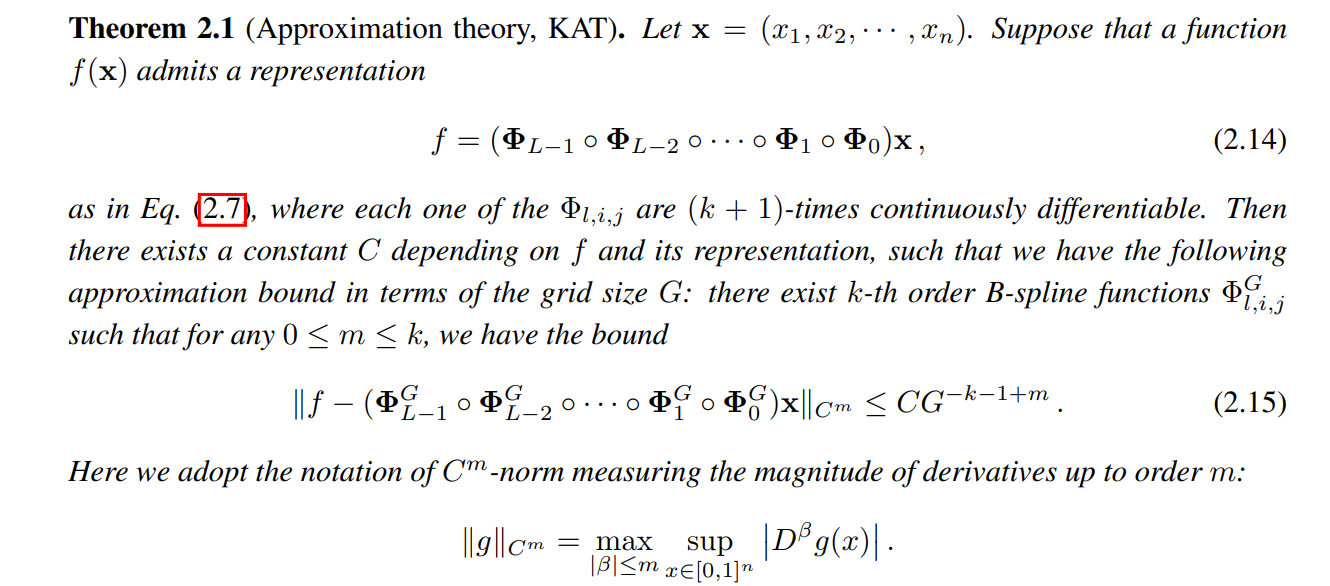
\includegraphics[height=5cm]{image copy 15.png}
    \end{figure}
\end{frame}
% Results --- --- --- --- --- --- --- --- --- --- --- 
\section{Results}
\begin{frame}
    \begin{itemize}
        \item different themes
        \item different themes
        \item different themes
        \item different themes
    \end{itemize}
\end{frame}


% --- Thank you slide ---
\begin{frame}
    \begin{center}
        {End}
        \vspace{1cm}

        MAS\\[1em]
    \end{center}
\end{frame}

\end{document}